\documentclass[submit]{harvardml}

% Put in your full name and email address.
\name{Anirudh Suresh}
\email{anirudh\_suresh@college.harvard.edu}

% List any people you worked with.
\collaborators{%
  John Doe,
  Fred Doe
}


% You don't need to change these.
\course{CS281-F17}
\assignment{Assignment \#0, v 1.0}
\duedate{5:00pm Sept. 8th}
\newcommand{\attr}[1]{\textsf{#1}}
\usepackage[OT1]{fontenc}
\usepackage[colorlinks,citecolor=blue,urlcolor=blue]{hyperref}
\usepackage[pdftex]{graphicx}
\usepackage{fullpage}
\usepackage{palatino}
\usepackage{amsfonts}
\usepackage{amsmath}
\usepackage{amssymb}
\usepackage{color}
\usepackage{todonotes}
\usepackage{listings}
\usepackage{common}
\usepackage{bm}
\usepackage{enumitem}
\usepackage{tikz}
\usepackage{xifthen}
\usepackage{soul}
\usepackage{url}
\usepackage[mmddyyyy,hhmmss]{datetime}
\definecolor{verbgray}{gray}{0.9}
% Some useful macros.
\newcommand{\R}{\mathbb{R}}
\newcommand{\E}{\mathbb{E}}
\newcommand{\cov}{\text{cov}}
\renewcommand{\v}[1]{\mathbf{#1}}

\begin{document}
\begin{center}
    {\Large Homework 0: Preliminary}
\end{center}

\subsection*{Introduction}

There is a mathematical component and a programming component to this homework.
Please submit your PDF and Python files to Canvas, and push all of your work
to your GitHub repository. If a question requires you to make any plots,
please include those in the writeup.

This assignment is intended to ensure that you have the background required for CS281,
and have studied the mathematical review notes provided in section.
You should be able to answer the problems below \textit{without} complicated calculations.
All questions are worth $70/6 = 11.\bar{6}$ points unless stated otherwise.

\newpage



%%%%%%%%%%%%%%%%%%%%%%%%%%%%%%%%%%%%%%%%%%%%%%%%%%%%%%%%
%%%%%%%%%%%%%%%%%% PROBLEM 1 %%%%%%%%%%%%%%%%%%%%%%%%%%%
%%%%%%%%%%%%%%%%%%%%%%%%%%%%%%%%%%%%%%%%%%%%%%%%%%%%%%%%
\section*{Variance and Covariance}
\begin{problem}
Let $X$ and~$Y$ be two independent random variables.

\begin{enumerate}[label=(\alph*)]
\item Show that the independence of~$X$ and~$Y$ implies that their
covariance is zero.

\item Zero covariance \textit{does not} imply independence between two
      random variables. Give an example of this.

\item For a scalar constant~$a$, show the following two properties:
\begin{align*}
  \E(X + aY) &= \E(X) + a\E(Y)\\
  \var(X + aY) &= \var(X) + a^2\var(Y)
\end{align*}
\end{enumerate}
\end{problem}

\section*{Solution}

\begin{enumerate}[label=(\alph*)]
    \item Using the standard definition of covariance,\[Cov(X,Y) = \E(X Y) - \mu_X \mu_Y.\] When X and Y are independent, $\E(X Y) = \E(X) \E(Y)$. Therefore,\[Cov(X,Y) = \E(X) \E(Y) - \mu_X \mu_Y = \mu_X \mu_Y - \mu_X \mu_Y = 0.\] Hence, the covariance of two independent random variables is $0$.
    \item Let us use $X$ and $Y = X^2$ as our two random variables. Clearly, $Y$ is not independent of $X$; its very value depends completely on the value of $X$. However, if we look at the covariance calculation,\[Cov(X,Y) = Cov(X,X^2) = \E(X X^2) - \mu_X \mu_{X^2} = \E(X^3) - 0 (\mu_{X^2}) = 0.\] Because $X$ and $X^3$ are symmetric about $X = 0$, their expectations are 0 for any range symmetric about the $y$-axis. Hence, though $X$ and $Y$ are inherently tied together in this example, they have zero covariance, indicating that zero covariance does not imply independence.
    \item Because of the independence of $X$ and $Y$,\[\E(X + aY) = \E(X) + \E(aY).\] Using the standard definition of covariance and realizing that since $a$ is a constant, $Cov(a,Y) = 0$,\[Cov(a,Y) = \E(aY) - a \mu_Y = 0\]\[\E(aY) = a \mu_Y = a \E(Y).\] Hence,\[\E(X + aY) = \E(X) + \E(aY) = \E(X) + a \E(Y).\]
    
    For the second property, we can use a definition of variance in terms of covariance.\[\var(X + aY) = \var(X) + 2 Cov(X,aY) + \var(aY) = \var(X) + 0 + \var(aY)\]\[\var(aY) = \E(a^2 Y^2) - (\E(aY))^2 = a^2 \E(Y^2) - (a \E(Y))^2 = a^2 (\E(Y^2) - (\E(Y))^2) = a^2 \var(Y).\] Thus,\[\var(X + aY) = \var(X) + \var(aY) = \var(X) + a^2 \var(Y).\]
\end{enumerate}

\newpage
%%%%%%%%%%%%%%%%%%%%%%%%%%%%%%%%%%%%%%%%%%%%%%%%%%%%%%%%
%%%%%%%%%%%%%%%%%% PROBLEM 2 %%%%%%%%%%%%%%%%%%%%%%%%%%%
%%%%%%%%%%%%%%%%%%%%%%%%%%%%%%%%%%%%%%%%%%%%%%%%%%%%%%%%
\section*{Densities}
\begin{problem}
Answer the following questions:
\begin{enumerate}[label=(\alph*)]
  \item Can a probability density function (pdf) ever take values greater than 1?
  \item Let $X$ be a univariate normally distributed random variable with mean 0
        and variance $1/100$. What is the pdf of $X$?
  \item What is the value of this pdf at 0?
  \item What is the probability that $X = 0$?
  \item Explain the discrepancy.
\end{enumerate}
\end{problem}

\section*{Solution}

\begin{enumerate}[label=(\alph*)]
    \item A PDF can certainly take values greater than $1$. For example, any random variable uniformly distributed over a range smaller than $1$ has a PDF that takes on values greater than $1$ in that range.
    \item $f(x) = \frac{1}{\sqrt{2 \pi (\frac{1}{100})}} \exp(-\frac{x^2}{2(\frac{1}{100})}) = \frac{10}{\sqrt{2 \pi}} \exp(-50 x^2)$
    \item $f(0) = \frac{10}{\sqrt{2\pi}}$
    \item $P(0) = \int_{0}^{0} f(x) dx = 0 $
    \item This is a continuous random variable, and thus, the probability that it is equal to any one discrete value is infinitesimally small. Hence, although $X=0$ is the obvious center of the distribution, it by itself has $0$ probability.
\end{enumerate}

\newpage
%%%%%%%%%%%%%%%%%%%%%%%%%%%%%%%%%%%%%%%%%%%%%%%%%%%%%%%%
%%%%%%%%%%%%%%%%%%%% PROBLEM 3 %%%%%%%%%%%%%%%%%%%%%%%%%
%%%%%%%%%%%%%%%%%%%%%%%%%%%%%%%%%%%%%%%%%%%%%%%%%%%%%%%%
\section*{Conditioning and Bayes' rule}
\begin{problem}
  Let $\v \mu \in \R^m$ and
  $\v \Sigma, \v \Sigma' \in \R^{m \times m}$.  Let $X$ be an
  $m$-dimensional random vector with
  $X \sim \mathcal{N}(\v \mu, \v \Sigma)$, and let $Y$ be a
  $m$-dimensional random vector such that
  $Y \given X \sim \mathcal{N}(X, \v \Sigma')$. Derive the
  distribution and parameters for each of the following.

\begin{enumerate}[label=(\alph*)]
  \item The unconditional distribution of $Y$.

  \item The joint distribution for the pair $(X,Y)$.

\end{enumerate}

Hints:
\begin{itemize}
\item You may use without proof (but they are good advanced exercises)
  the closure properties of multivariate normal distributions. Why is
  it helpful to know when a distribution is normal?
\item Review Eve's and Adam's Laws, linearity properties of
  expectation and variance, and Law of Total Covariance.

\end{itemize}

\end{problem}

\section*{Solution}

\begin{enumerate}[label=(\alph*)]
    \item Using Adam's Law,\[\E(Y) = \E(\E(Y \given X)) = \E(X) = \v \mu.\] Using Eve's Law,\[\var(Y) = \E(\var(Y \given X)) + \var(\E(Y \given X)) = \E(\v \Sigma') + \var(X) = \v \Sigma' + \v \Sigma.\]
    
    $Y \given X \sim \mathcal{N}$, and through the closure properties of the multivariate normal (if the conditional on a Gaussian is Gaussian, the marginal should similarly be Gaussian), $Y \sim \mathcal{N}$. Thus,\[Y \sim \mathcal{N}(\v \mu,\v \Sigma + \v \Sigma').\]
    
    \item We know that the joint distribution for the pair $(X,Y)$ given that both variables have a marginal normal distribution and the conditional is normal is \[(X,Y) \sim \mathcal{N}(\left( \begin{array}{c} \mu \\ \mu \end{array} \right),\left( \begin{array}{cc} \var(X) & Cov(X,Y) \\ Cov(Y,X) & \var(Y) \end{array} \right)).\] We can compute the covariance from the definition of covariance \[Cov(X,Y) = \E(XY) - \E(X)\E(Y).\] Via Adam's Law,\[= \E(\E(XY \given X)) - (\mu)(\mu)\]\[= \E(X^2) - \mu^2\]\[\E(X^2) = \var(X) + (\E(X))^2 = \Sigma + \mu^2\] Thus,\[Cov(X,Y) = \Sigma + \mu^2 - \mu^2 = \Sigma.\] Hence,\[(X,Y) \sim \mathcal{N}(\left( \begin{array}{c} \mu \\ \mu \end{array} \right),\left( \begin{array}{cc} \Sigma & \Sigma \\ \Sigma & \Sigma + \Sigma' \end{array} \right))\]
\end{enumerate}

\newpage
%%%%%%%%%%%%%%%%%%%%%%%%%%%%%%%%%%%%%%%%%%%%%%%%%%%%%%%%
%%%%%%%%%%%%%%%%% PROBLEM 4 %%%%%%%%%%%%%%%%%%%%%%%%%%%%
%%%%%%%%%%%%%%%%%%%%%%%%%%%%%%%%%%%%%%%%%%%%%%%%%%%%%%%%
\section*{I can Ei-gen}
\begin{problem}
    Let $\v X \in \R^{n \times m}$.
    \begin{enumerate}[label=(\alph*)]
        \item What is the relationship between the $n$ eigenvalues
              of $\v X \v X^T$ and the $m$ eigenvalues of $\v X^T \v X$?
        \item Suppose $\v X$ is square (i.e., $n=m$) and symmetric.
              What does this tell you about the eigenvalues of $\v X$?
              What are the eigenvalues of $\v X + \v I$, where $\v I$ is the identity matrix?
        \item Suppose $\v X$ is square, symmetric, and invertible.
			  What are the eigenvalues of $\v X^{-1}$?
	\end{enumerate}
	Hints:
	\begin{itemize}
		\item Make use of singular value decomposition and the properties
			  of orthogonal matrices. Show your work.
		\item Review and make use of (but do not derive) the spectral theorem.
	\end{itemize}
\end{problem}

\section*{Solution}

\begin{enumerate}[label=(\alph*)]
    \item Using the definition of an eigenvalue-eigenvector pair,\[\v X^T \v X \v{v_1} = \lambda \v{v_1}.\] Left multiplying each side of the identity above by $\v X$,\[\v X \v X^T \v X \v{v_1} = \lambda \v X \v{v_1}\]\[\v X \v X^T \v{v_2} = \lambda \v{v_2},\] where $\v{v_2} = \v X \v{v_1}$ reveals that $\v X \v X^T$ and $\v X^T \v X$ share the same eigenvalues.
    
    \item If $\v X$ is square and symmetric, it has the same number of (not necessarily distinct) eigenvalues as its dimensions/rank. Hence, it will have $n$ real (if all its entries are real) eigenvalues. In addition,\[\v X = \v X^T.\] Thus, the eigenvalues of $\v X$ are the same as the eigenvalues of $\v X^T$. If we denote the eigenvalues of $\v X$ as $\lambda_i$, $i \in [1,n]$ and the eigenvalues of $\v X + \v I$ as $\kappa_i$, $i \in [1,n]$,\[\kappa_i = \lambda_i + 1, i \in [1,n].\]
    
    \item Via the spectral theorem,\[\v X = \v Q^{-1} \v D \v Q,\] where $\v Q$ is an orthogonal matrix and $\v D$ is a diagonalized form of $\v X$. $\v X^{-1}$. Then, we can immediately see that \[\v X^{-1} = \v Q^{-1} \v D^{-1} \v Q.\] Since $\v D$ is a diagonal matrix, $\v D^{-1}$ is as well, with its diagonal entries the reciprocals of their respective counterparts in $\v D$. Since the diagonal matrix $\v D$ contains the eigenvalues of $\v X$. $\v D^{-1}$ must contain the eigenvalues of $\v X^{-1}$. Hence, given eigenvalues of $\v X$ $\lambda_i, i \in [1,n]$, $\v X^{-1}$ must have eigenvalues $\frac{1}{\lambda_i}, i \in [1,n]$. For this to be the case, $\lambda_i \neq 0$ for all $i \in [1,n]$, which is the case since $\v X$ is specified to be invertible.
    
\end{enumerate}

\newpage
%%%%%%%%%%%%%%%%%%%%%%%%%%%%%%%%%%%%%%%%%%%%%%%%%%%%%%%%%%
%%%%%%%%%%%%%%%%%%% PROBLEM 5 %%%%%%%%%%%%%%%%%%%%%%%%%%%%
%%%%%%%%%%%%%%%%%%%%%%%%%%%%%%%%%%%%%%%%%%%%%%%%%%%%%%%%%%
\section*{Vector Calculus}
\begin{problem}
  Let $\v x, \v y \in \R^m$ and $\v A \in \R^{m \times m}$. Please derive from
  elementary scalar calculus the following useful properties. Write
  your final answers in vector notation.
\begin{enumerate}[label=(\alph*)]
    \item What is the gradient with respect to $\v x$ of $\v x^T \v y$?
    \item What is the gradient with respect to $\v x$ of $\v x^T \v x$?
    \item What is the gradient with respect to $\v x$ of $\v x^T \v A \v x$?
\end{enumerate}
\end{problem}

\section*{Solution}

\begin{enumerate}[label=(\alph*)]
    \item Using the symbol $:=:$ to indicate the scalar ``equivalent" of a particular vector notation term,\[\v x^T \v y = \sum_{i=1}^{m} x_i y_i :=: x y\]\[\frac{\partial \v x^T \v y}{\partial \v x} = \frac{\partial(\sum_{i=1}^{m} x_i y_i)}{\partial \v x} :=: \frac{\partial(x y)}{\partial x}\]\[\frac{\partial \v x^T \v y}{\partial \v x} = \v y\]
    
    \item \[\v x^T \v x = \sum_{i=1}^{m} x_i x_i :=: x x = x^2\]\[\frac{\partial \v x^T \v x}{\partial \v x} = \frac{\partial(\sum_{i=1}^{m} x_i x_i)}{\partial \v x} :=: \frac{\partial x^2}{\partial x}\]\[\frac{\partial \v x^T \v x}{\partial \v x} = 2 \v x\]
    
    \item Using results from the previous two parts and the product rule,\[\frac{\partial \v x^T \v A \v x}{\partial \v x} = \frac{\partial(\sum_{i=1}^{m} x_i (\sum_{j=1}^{m} \sum_{k=1}^{m} A_{j,k} x_k)_i)}{\partial \v x} = \frac{\partial(\sum_{j=1}^{m} \sum_{k=1}^{m} A_{j,k} x_k x_j)}{\partial \v x}\]\[\partial(\v x^T \v A \v x)=(\v{\partial x})^T \v A \v x + \v x \v A \v{\partial x} = (\v{\partial x})^T \v A \v x + (\v{\partial x})^T \v A^T \v x\]\[=(\v{\partial x})^T (\v A + \v A^T) \v x = \v x^T (\v A + \v A^T) \v{\partial x}\] Therefore,\[\frac{\partial \v x^T \v A \v x}{\partial \v x} = \v x^T (\v A + \v A^T).\]
    
\end{enumerate}

\newpage
%%%%%%%%%%%%%%%%%%%%%%%%%%%%%%%%%%%%%%%%%%%%%%%%%%%%%%%%%%%%
%%%%%%%%%%%%%%%%%%%%% PROBLEM 7 %%%%%%%%%%%%%%%%%%%%%%%%%%%%
%%%%%%%%%%%%%%%%%%%%%%%%%%%%%%%%%%%%%%%%%%%%%%%%%%%%%%%%%%%%
\section*{Gradient Check}
\begin{problem}
  Often after finishing an analytic derivation of a gradient, you will
  need to implement it in code.  However, there may be mistakes -
  either in the derivation or in the implementation. This is
  particularly the case for gradients of multivariate functions.

  \air

  \noindent One way to check your work is to numerically estimate the gradient
  and check it on a variety of inputs. For this problem we consider
  the simplest case of a univariate function and its derivative.  For
  example, consider a function $f(x): \mathbb{R} \to \mathbb{R}$:
$$\frac{d f}{d x} = \underset{\epsilon \to 0} \lim \frac{f(x + \epsilon) - f(x - \epsilon)}{2 \epsilon}$$
\noindent A common check is to evaluate the right-hand side for a small value of
$\epsilon$, and check that the result is similar to your analytic
result.\\

\smallskip

\noindent In this problem, you will implement the analytic and numerical derivatives of the function \[f(x) = \cos(x) + x^2 + e^x.\]

\begin{enumerate}
  \item Implement \texttt{f} in Python (feel free to use whatever \texttt{numpy} or \texttt{scipy} functions you need):
  \begin{lstlisting}[language=python]
  def f(x):

  \end{lstlisting}
  \item Analytically derive the derivative of that function, and implement it in Python:
  \begin{lstlisting}[language=python]
  def grad_f(x):

  \end{lstlisting}
  \item Now, implement a gradient check (the numerical approximation to the derivative), and by plotting, 
        show that the numerical approximation approaches the analytic as \texttt{epsilon} 
        $\to 0$ for a few values of $x$:
  \begin{lstlisting}[language=python]
  def grad_check(x, epsilon):

  \end{lstlisting}
\end{enumerate}
\end{problem}

\section*{Solution}

\begin{enumerate}
    \item See Python script
    \item \[f'(x) = -\sin(x) + 2x + e^x\] See Python script for implementation
    \item See Python script for implementation; the plots for $7$ different values of $x$ below clearly reveal that as $\epsilon \rightarrow 0$, the difference between the analytic and numerical expressions for the gradient converges to $0$.
    
    \begin{center}
        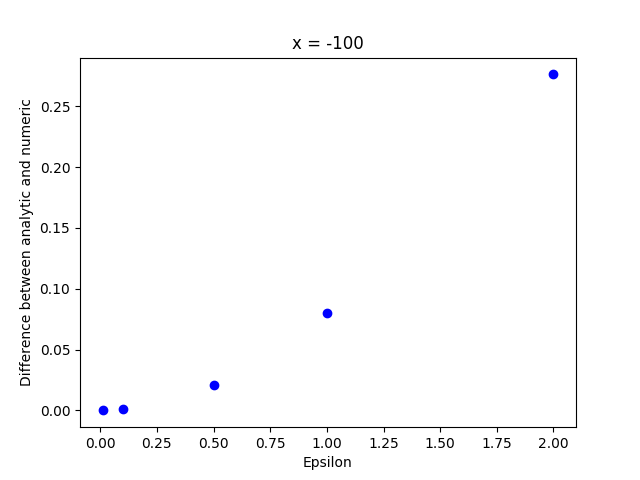
\includegraphics[width=0.6\textwidth]{x-100}\\
        Gradient check for x = -100
    \end{center}
    \begin{center}
        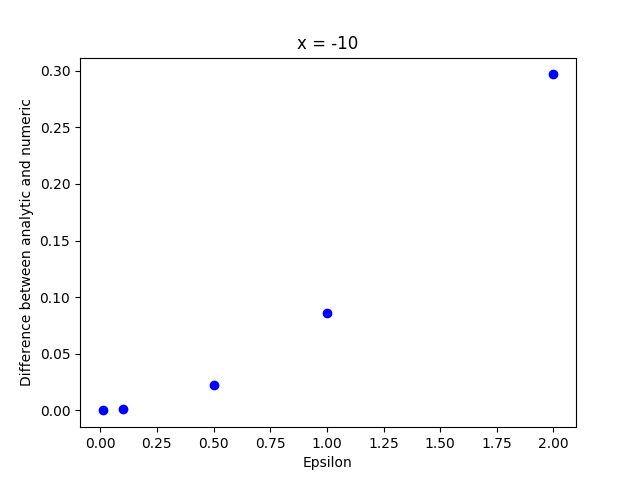
\includegraphics[width=0.6\textwidth]{x-10}\\
        Gradient check for x = -10
    \end{center}
    \begin{center}
        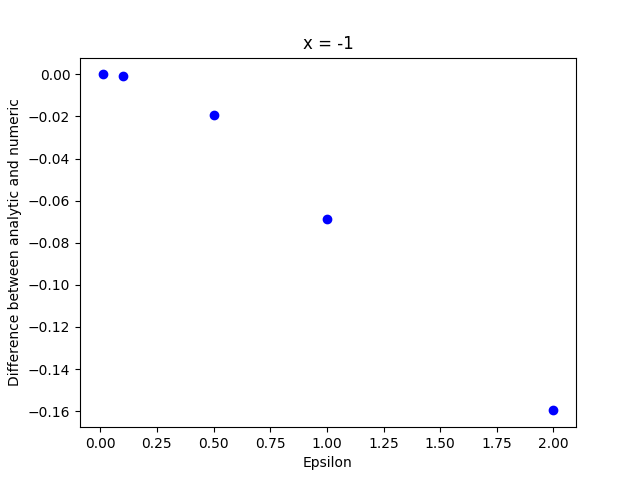
\includegraphics[width=0.6\textwidth]{x-1}\\
        Gradient check for x = -1
    \end{center}
    \begin{center}
        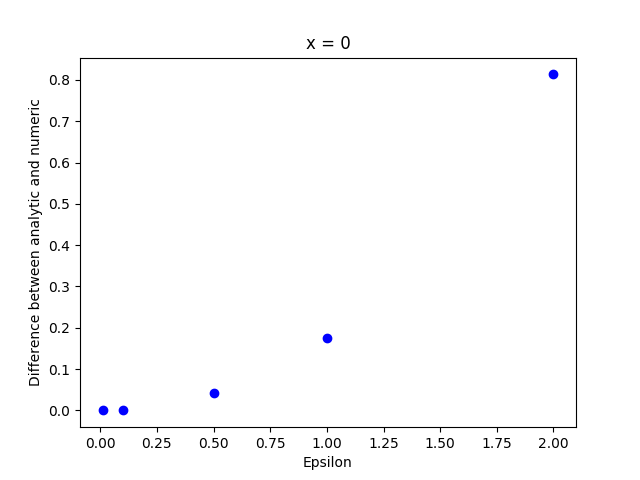
\includegraphics[width=0.6\textwidth]{x0}\\
        Gradient check for x = 0
    \end{center}
    \begin{center}
        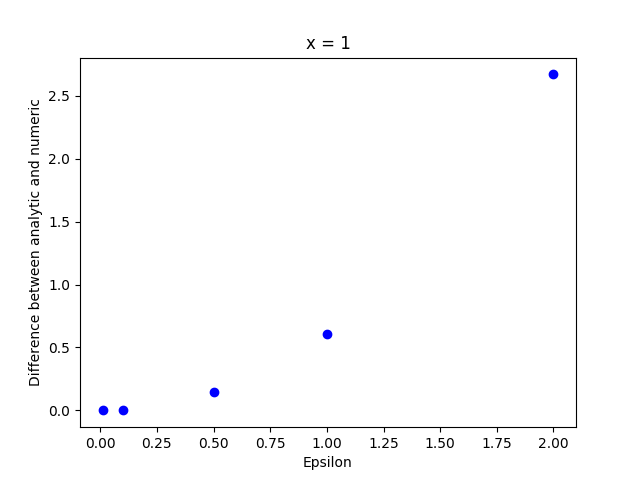
\includegraphics[width=0.6\textwidth]{x1}\\
        Gradient check for x = 1
    \end{center}
    \begin{center}
        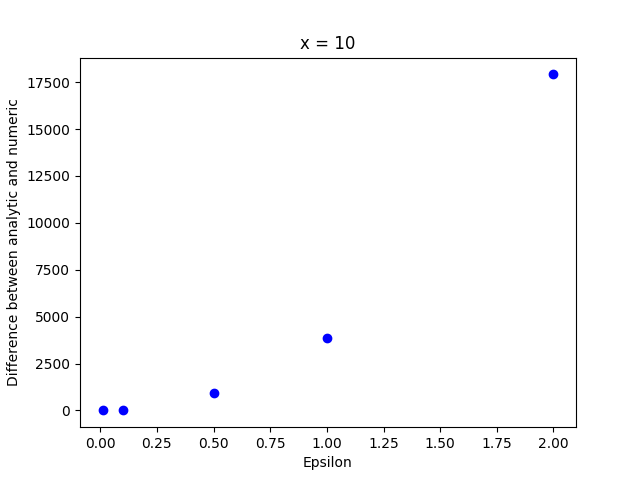
\includegraphics[width=0.6\textwidth]{x10}\\
        Gradient check for x = 10
    \end{center}
    \begin{center}
        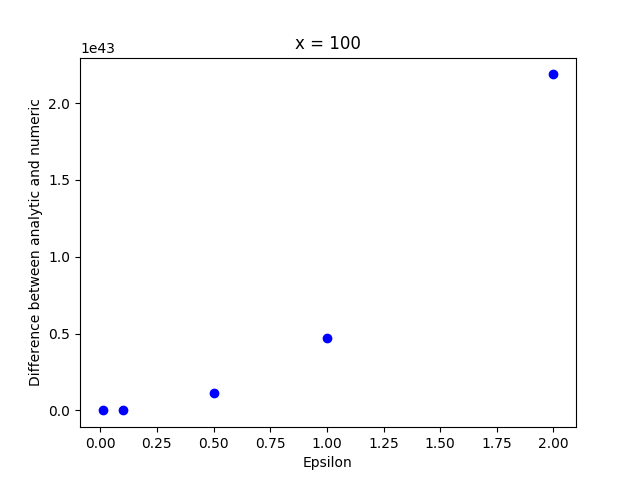
\includegraphics[width=0.6\textwidth]{x100}\\
        Gradient check for x = 100
    \end{center}
\end{enumerate}

\end{document}
